\chapter{System Design} \label{ch:design}

The requirements elicitation and the system design of the Swiss Educhain service proved to be a challenging but quite rewarding process. Previous work conducted in \cite{Gres18} was taken into consideration, but a greenfield approach was chosen. The initial requirements were re-evaluated and complemented with new functional and non-functional requirements, which were refined as implementation progressed. Research, design and implementation phases, entailed valuable interactions with stakeholders (e.g. workshop with the SWITCH edu-ID  program lead Christoph Graf, communication with UZH IdP (Identity Provider) administrator August Yannikis) and reaching out to the open source technical communities to comprehend how to best take advantage of the latest features, when documentation deemed to be insufficient \cite{shib-user-group-question}, \cite{stackoverflow-corda-service}, \cite{stackoverflow-corda-accounts}. \\
In Section \ref{sec:stakeholders}, the main stakeholders are identified, architectural requirements are elicited and produced, split into two distinct categories, functional and non-functional. Section \ref{sec:design-architecture} lists the different high-level design options for the Swiss Educhain service, the chosen solution, as well as a proposal for the overall governance model. Finally, Section \ref{sec:iam-design} is entirely focused on the identity and access management (IAM) part of Swiss Educhain and enumerates the different candidate approaches complemented by their individual evaluation, a detailed presentation of the engineered solution and the reasoning behind each decision.

\section{Stakeholders} \label{sec:stakeholders}

\emph{This is joint text with Simon M{\"u}ller \cite{mueller20}.}

Based on the stakeholder analysis conducted in \cite{Gres18}, stakeholders are analyzed from a technical perspective and mapped to different roles of the Swiss Educhain system. The main stakeholders and participants identified are:

\begin{description}
	\itemsep0em
	\item[Swiss Educhain Governance Body] \hfill \\
	The Swiss Educhain is governed from the UZH Blockchain Center \cite{noauthor_uzh_nodate} as a Free and Open Source Software (FOSS) project. The UZH Blockchain Center has the responsibility to onboard Issuing Organizations to the service.
	
	\item[Issuing Organization] \hfill \\
	Issuing Organization can be any educational institution or company that has been onboarded to the service and is given the right to issue diplomas, certificates of work history or other credentials that can be independently verified and included in a recipient's CV (Curriculum Vitae) or resume.
	
	\item[Issuer] \hfill \\
	The \texttt{Issuer} is an individual that is officially associated with an issuing organization and has been granted the right to issue digital certificates on behalf of this organization.
	
	\item[Recipient] \hfill \\
	\texttt{Recipient} is any individual that has an account in the Swiss Educhain service, receives educational or other credentials and can be associated with one or more Issuing Organizations. Each \texttt{Recipient} holds a single Swiss Educhain account that is mapped to only one real world identity.
	
	\item[System Administrator] \hfill \\
	The System Administrator is responsible for user administration, system maintenance and rollout of new system versions. The System Administrator has root access but has no right to issue credentials.
	
	
	\item[Verifier] \hfill \\
	Verifier is anyone that verifies a credential using the public permissionless blockchain. Verifiers are completely anonymous as they can verify any credential independently.
		
	\item[Contributor] \hfill \\
	Contributor is anyone that contributes to the project in a technical or non-technical fashion. Contributors include developers and extend to persons that add value to the project via any activity such as performing beta testing, writing documentation, reporting bugs, participating in discussions etc. 
	
\end{description}

\emph{This ends the text jointly written with Simon M{\"u}ller \cite{mueller20}.}


\section{Requirements} \label{ssec:architectural-requirements}

\emph{This is joint text with Simon M{\"u}ller \cite{mueller20}.}

In addition to the requirements identified in \cite{Gres18} the requirements in Sections \ref{ssec:func-req} and \ref{ssec:nonfunc-reqs} have been elicited.

\subsection{Functional Requirements} \label{ssec:func-req}


\begin{table}[h!]
	\centering
	\resizebox{\textwidth}{!}{%
		\begin{tabular}{| l | l |}
			\hline
			\textbf{Requirement}	& \textbf{Description} \\ \hline
			RQ1	& Only authorized individuals are allowed to issue diplomas. \\ \hline
			RQ2	& Diploma data should be confidential to its \texttt{Recipients}.  \\ \hline
			RQ3	& Process of issuing and verifying diplomas should abstract technical complexities.  \\ \hline
			RQ4	& Multiple diplomas should be processable in batch.  \\ \hline
			RQ5	& Verification capabilities should be accessible to anyone.  \\ \hline
			RQ6	& Diplomas should be verified autonomously.  \\ \hline
			RQ7	& Graduates should receive their diplomas in a digital format.  \\ \hline
		\end{tabular}%
	}
	\caption{Initial Educhain Requirements based on \cite{educhain-architecture}}
	\label{tab:educhain-requirements-jerinas}
\end{table}

Further functional requirements proposed for the Swiss Educhain project are:

\begin{table}[h!]
	\centering
	\begin{tabularx}{\textwidth}{| l | X |}
		\hline
		\textbf{Requirement}	& \textbf{Description} \\ \hline
		RQ8 & \texttt{Recipients} should have a unique identification. \\ \hline
		RQ9 & \texttt{Recipients} should be the only ones that have the right to disclose issued credentials. \\ \hline
		RQ10 & \texttt{Recipient's} account should persist over time and be independent of any association with an Issuing Organization.  \\ \hline
		RQ11 & Registration needs identity verification. \\ \hline
		RQ12 & \texttt{Issuers} should be able to revoke diplomas. \\ \hline
		RQ13 & The governance model of the Swiss Educhain system must be defined.  \\ \hline
		RQ14 & Issuing should create an unchangeable audit trail. \\ \hline
		RQ15 & Data owner is responsible for data backup. System should provide an option for a participants' data to be exported. \\ \hline
		RQ16 & Multisig transactions should be possible. \\ \hline
		RQ17 & System processes data in a text-based format.  \\ \hline
		RQ18 & Allow for identity details to change (e.g. name, address). \\ \hline
		RQ19 & The process to onboard Issuing Organisations to the Swiss Educhain service needs to be examined and defined. \\ \hline
		RQ20 & User accounts need to be associated with one or more Issuing Organizations.  \\ \hline
		
	\end{tabularx}
	\caption{Swiss Educhain Functional Requirements}
	\label{tab:func-reqs}
\end{table}

Some of the functional requirements are described in more detail:

\begin{description}
	\itemsep0em
	\item[RQ8] \hfill \\ Any \texttt{Recipient} should be uniquely identified and use a single account that is used to receive diplomas, certificates, certificate of employment etc. issued from multiple issuing organizations.
	
	\item[RQ9] \hfill \\ Issued diplomas and other digital credentials should be entirely owned by the recipient and not the institution/company that issues them. This will allow for complete control of someone's data and enable a granular voluntary peer-to-peer read-only disclosure (temporary or permanent).
	
	\item[RQ10] \hfill \\ The cease of operation of any Issuing Organization should not affect the \texttt{Recipient's} account, it must also be ensured that no individual other than the System Administrator has the ability to suspend or lock a \texttt{Recipient's} account.
	
	\item[RQ11] \hfill \\ The user account creation process (or user registration) needs to be defined, and map one single real-world identity to a unique digital identity. As part of this process the need for a Know-Your-Customer (KYC) process or identity verification should be examined.
	
	\item[RQ12] \hfill \\ \texttt{Issuers} of a digital credential must be able to revoke it if there is proof that the \texttt{Recipient} acquired it maliciously or by falsifying information.
	
	\item[RQ16] \hfill \\
	Multisig refers to the technical ability for multiple parties to sign a transaction.
	
	\item[RQ17] \hfill \\ Any produced files such as PDFs (Portable Document Format) must be converted to a text-based format (i.e. using base64 conversion) and included in a JSON (JavaScript Object Notation) file/structure.
	
	\item[RQ18] \hfill \\ \texttt{Recipient} should be able to request an update to his data.
	
	\item[RQ20] \hfill \\ The association of user accounts to one or more Issuing Organizations must be defined, this includes the assignment of specific roles for members within a certain Organization such as credential \texttt{Issuer} and \texttt{Recipient}.
\end{description}


\subsection{Non-Functional Requirements} \label{ssec:nonfunc-reqs}

The Swiss Educhain system is intended to provide a service to a plethora of organizations such as universities, government departments and employers of different sizes, in diverse jurisdictions and of varying technology maturity level. This creates the need for a system that fulfills these non-functional requirements:

\newpage

\begin{table}[H]
	\centering
	\begin{tabularx}{\textwidth}{| l | X |}
		\hline
		\textbf{Requirement}	& \textbf{Description} \\ \hline
		RQ21 & Verifier must be able to verify the diploma even when the private environment is not available. \\ \hline
		RQ22 & Easy to use from a user perspective, with a simple UX/UI and straightforward functionality. \\ \hline
		RQ23 & Easy to install, configure, deploy, operate, monitor and maintain from a System Administrator's perspective. \\ \hline
		RQ24 & Uses technologies that are freely available, popular, well-established and mature. \\ \hline
		RQ25 & Has as few as possible technology requirements and dependencies both in terms of hardware and software. \\ \hline
		RQ26 & Can be easily integrated with existing IT infrastructure and is cross-platform compatible. \\ \hline
		RQ27 & Is not dependent on state-of-the-art technologies such as Containers, Cloud etc. \\ \hline
		RQ28 & System should support multiple issuing organizations. \\ \hline
		%RQ30 & Can be extended to deploy nodes of the network to mobile devices. \\ \hline
		RQ29 & High-level access control must be defined for the different kind of identities participating in the system. %Which account has access to what kind of functionality and what part of the system. Who can trigger which actions etc.
		\\ \hline
		RQ30 & Can be modularly enhanced by existing functionality. \\ \hline
		RQ31 & Data that are disclosed peer-to-peer should not be broadcasted. \\ \hline
		%RQ33 & Ensures data integrity. \\ \hline
		RQ32 & All transactions in the system should be signed and the identity of any action initiator should be verifiable. \\ \hline
		
		
	\end{tabularx}
	\caption{Swiss Educhain Non-Functional Requirements}
	\label{tab:non-func-reqs}
\end{table}

\emph{This ends the text jointly written with Simon M{\"u}ller \cite{mueller20}.}

\section{Architecture} \label{sec:design-architecture}

This Section discusses the chosen high-level architecture for Swiss Educhain. This work was done in close collaboration with \cite{mueller20} using common decision criteria, the IAM specific architecture is explained in Section \ref{sec:iam-design}. Some important factors and goals taken into consideration during this design phase include:

\begin{description}
	\itemsep0em
	\item\textbf{Requirements fulfillment}  \hfill \\ 
	The chosen solution should partially or completely fulfill the majority of the architectural requirements identified in Section \ref{ssec:architectural-requirements}.
	\item\textbf{Real-world application}  \hfill \\ 
	The Swiss Educhain service is planned to be eventually deployed as a real-world service for members of academia, with the aspiration to serve additional use cases in the future. In contrast to other projects or proof-of-concepts that are created as part of a thesis or an academic project, this work will continue to be developed and improved upon until it is production ready.
	\item\textbf{Privacy, Security and Verifiability}  \hfill \\ 
	Swiss Educhain must handle sensitive user data, thus, it is crucial that information is stored and transferred securely and disclosed strictly on a need-to-know basis only. Actions such as issuing or blacklisting diplomas must be auditable, with the identity of any action initiator easily verifiable.
	\item\textbf{Simple development and operation}  \hfill \\ 
	As students are the main contributors and the service will be operated under the academic umbrella, it is essential that no specialized knowledge is required to be able to develop, maintain and operate the service. This would also mean that a strong preference to open source, well documented and widely adopted technologies should be given.
	\item\textbf{Extensible modular architecture}  \hfill \\ 
	New features' development, easy integration with existing or future external components and uncomplicated co-hosting of the service with other systems should be enabled. To achieve this goal, a modular loosely coupled architecture should be designed, so components can interact using clearly defined interfaces that encapsulate and hide the chosen functionality implementation(s).
\end{description}

Based on the guidelines and goals mentioned above, an appropriate solution is chosen in Section \ref{ssec:arch-solution} and the implementation details are mentioned in Chapter \ref{ch:implementation}.

\subsection{Candidate Solutions} \label{ssec:design-candidate-solutions}

After conducting initial research and taking into consideration possible technical solutions and available technologies, two major options were identified for the Swiss Educhain service which are explained in this Section.

\subsubsection{Governance Model} \label{ssec:design-governance-model}

\emph{This is joint text with Simon M{\"u}ller \cite{mueller20}.}

The Swiss Educhain ecosystem is comprised of a variety of institutions and stakeholders as identified in \ref{sec:stakeholders}. This creates challenges and different options for the governance model to be chosen.

Two different governance and operational models have been determined:

\begin{description}
	\itemsep0em
	\item[Option 1: Global Network] \hfill \\
	A global network is deployed, where different organizations are onboarded. A process to identify accredited institutions and to allow them to participate in the system as \texttt{Issuers} must be defined and explored both in technical and non-technical aspects. The system is operated and governed by the UZH Blockchain Center which is responsible for administration, support and new functionality.
	
	\begin{description}
		\itemsep0em
		\item[Advantages] \hfill \\
		Only one user account for each \texttt{Recipient}. \hfill \\
		Unified update and upgrade rollout. \hfill \\
		Low administration and operational effort.	 \hfill 
		\item[Disadvantages] \hfill \\
		Forced update and upgrade policy. \hfill \\
		More complex identity management. \hfill 		
	\end{description}
	
	\item [Option 2: Per-institution Network] \hfill \\ 
	Each institution deploys and operates an independent instance of the FOSS Swiss Educhain service. The service is entirely operated and governed by each institution which is responsible for administration, support and new functionality.
	
	\begin{description}
		\itemsep0em
		\item[Advantages] \hfill \\
		More control over the system. \hfill \\
		Independent update and upgrade rollouts. \hfill 
		
		\item[Disadvantages] \hfill \\
		High administration and operational effort. \hfill \\
		Users need new account for each institution. \hfill \\
		Institution's cease of operation results in unexpected system termination. \hfill 
	\end{description}
\end{description}

After weighing advantages and disadvantages between option 1 and option 2, the Global Network governance and operational model was the preferred choice. A global network from a technical perspective simplifies the deployment and operation of the system. Assuming that the Swiss Educhain service will be adopted by multiple institutions a global standardized network will simplify the user administration and reduce significantly the overhead of operating multiple parallel instances of the system. 

\emph{This ends the text jointly written with Simon M{\"u}ller \cite{mueller20}.}

\subsection{Architecture Solution} \label{ssec:arch-solution}

\emph{This is joint text with Simon M{\"u}ller \cite{mueller20}.}

After the initial analysis of the previously elicited requirements the resulting Swiss Educhain high-level architecture is depicted in Figure \ref{fig:arch-full}.

\begin{figure}[!h]
	\centering
	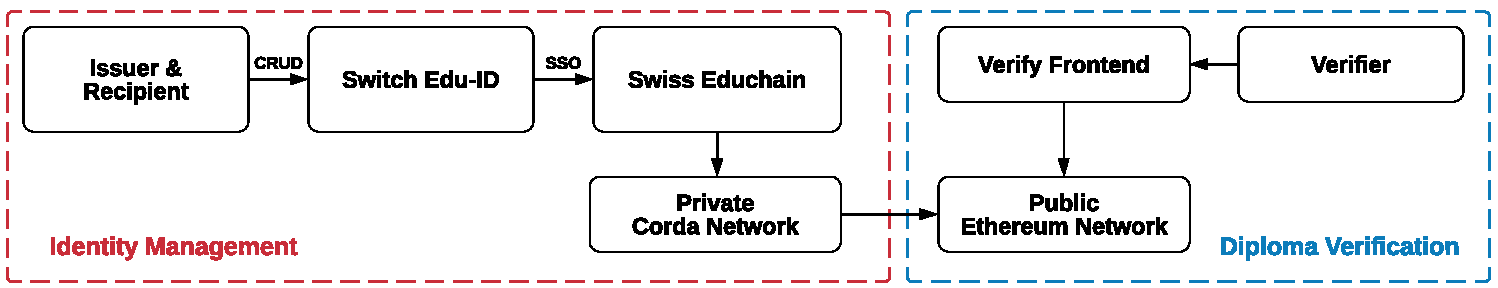
\includegraphics[width=\textwidth]{figs/ch4/arch-full}
	\caption{Swiss Educhain high-level architecture.}
	\label{fig:arch-full}
\end{figure}

The high-level architecture as shown in \ref{fig:arch-full} illustrates the logically separated steps and processes entailed in the end-to-end issuance and verification of a diploma. 

Initially, the diploma \texttt{Issuer} and \texttt{Recipient} register to the Swiss Educhain service with their SWITCH edu-ID account which integrates through the Shibboleth web single sign-on (SSO) implementation. The Swiss Educhain service leverages Spring Boot and the Corda distributed ledger (DL) to execute core functionality, such as, executing signed transactions, storing account and diploma information in states, and permitting \texttt{Issuers} to issue diplomas to \texttt{Recipients}. \\
Corda was chosen as the private permissioned blockchain due to the excellent compatibility with other system components, such as Apache and the AJP connector. Futhermore, it is written in Kotlin same as the Spring Boot webserver simplifying development and it offers extensive up-to-date documentation. Then, the issued diplomas can be hashed and published, individually or in batches, to the public Ethereum ledger via a Solidity smart contract which offers additionally the option to blacklist an already published diploma. As a last step in the issuance process verification can occur independently and anonymously by any person or organization.

To achieve the minimum required functionality for a proof-of-concept implementation as described in Section \ref{ssec:mvp-requirements}, a plethora of components and different technologies were combined. A detailed architecture of the Swiss Educhain components is depicted below in Figure \ref{fig:arch-educhain}.

\begin{figure}[H]
	\centering
	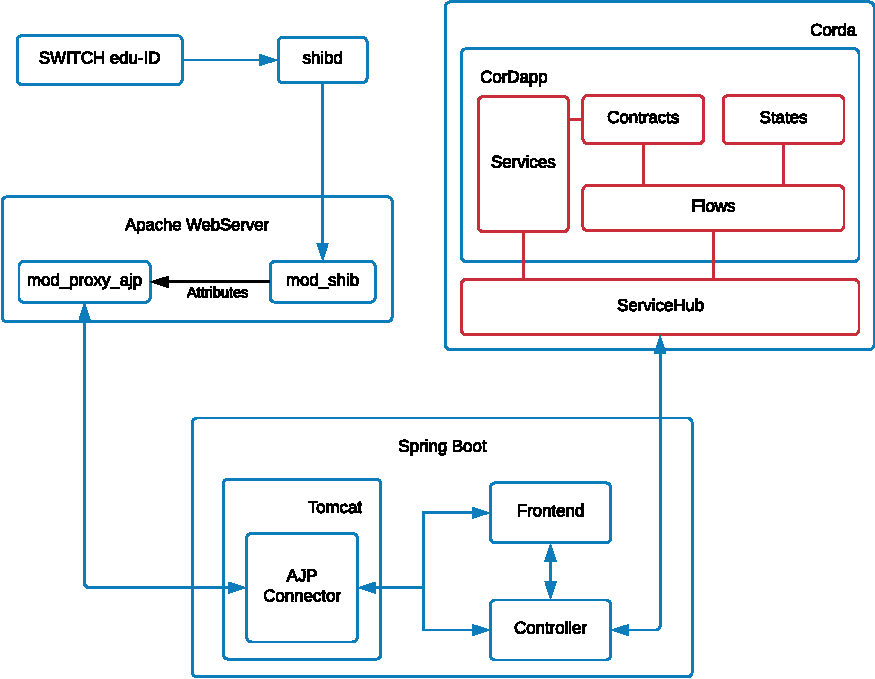
\includegraphics[width=0.8\textwidth]{figs/ch4/arch-educhain}
	\caption{Swiss Educhain component architecture.}
	\label{fig:arch-educhain}
\end{figure}

%The Swiss Educhain component architecture is depicted in 
Figure \ref{fig:arch-educhain} outlines the inner workings of the Swiss Educhain application component and depicts in detail all interactions down to the module level. 

As it can be seen in Figure \ref{fig:arch-educhain}, the Swiss Educhain service is dependent on the account information provided by SWITCH edu-ID. SWITCH edu-ID relays attributes from a logged-in user to \texttt{shibd}, the Shibboleth daemon service, through the \texttt{mod\_shib} the Apache Webserver Shibboleth module. With this configuration in place, Apache is able to disclose the user account attributes via the Apache JServ Protocol (AJP) over the \texttt{mod\_proxy\_ajp} module when requested by the Spring Boot application server. An embedded Tomcat server resides inside the Spring Boot application that is listening to and serving all call requests, over the custom AJP Connector, from and to the Apache Webserver. The embedded Tomcat server hosts the Frontend over which a logged-in user interacts with the Swiss Educhain service. Additionally, in the Spring Boot application relies the Controller which exposes various RESTful endpoints to the Frontend and the Tomcat server. \\
When the controller receives a request that requires a connection to Corda it calls the Corda ServiceHub via a Remote Procedure Call (RPC) operation. Within Corda, ServiceHub is the main orchestrating entity can be viewed as an entry point. It routes all requests to the appropriate service or flow that are part of the Corda Decentralized Application (CorDapp). Services and flows execute transactions based on the contract rules, store or update information on states and cryptographically ensure the overall system privacy, security and actions verifiability.

\emph{This ends the text jointly written with Simon M{\"u}ller \cite{mueller20}.}

\subsection{MVP Functionality} \label{ssec:mvp-requirements}

\emph{This is joint text with Simon M{\"u}ller \cite{mueller20}.}

The following functionality has been identified as the minimum required for a PoC version of Swiss Educhain:

\begin{description}
	\itemsep0em
	\item [Identity management] \hfill \\
	Two types of identities should be supported, \texttt{Issuers} and \texttt{Recipients}. \hfill \\
	Define process of creating a new account. \hfill \\
	Define data structures for the Educhain account data. \hfill \\
	Define access control rules for general access to the service. \hfill \\
	Define application level access control for \texttt{Issuers}. \hfill \\
	Fetch student details to create Corda identities. \hfill \\
	Detect student detail changes and update Educhain account automatically. \hfill
	
	\item [Data Structures] \hfill \\
	Define an appropriate data structure for storing data related to a diploma. \hfill \\
	Allow digital diploma hashing and publishing on a public blockchain. \hfill \\
	Allow existing diplomas to be digitally signed and published. \hfill \\
	Publish diplomas in batch. \hfill \\
	Blacklist diplomas. \hfill 
	
	\item [Web Interface] \hfill \\
	Issue diploma by uploading JSON. \hfill \\
	View received diplomas (all users). \hfill \\
	View issued diplomas (only \texttt{Issuers}). \hfill \\
	\texttt{Issuer} should be able to perform all actions from the frontend. \hfill \\
	Provide a simple login and logout interface. \hfill 
	
	\item [Operations] \hfill \\
	Define build, installation and deployment process. \hfill \\
	Encryption for data in transit and data at rest. \hfill \\
	Cross-platform compatibility. \hfill 
\end{description}

\emph{This ends the text jointly written with Simon M{\"u}ller \cite{mueller20}.}

\section{Identity and Access Management} \label{sec:iam-design}

With Corda as the chosen private permissioned blockchain technology to be used, an end-to-end IAM system must be designed, implemented and tightly integrated to offer appropriate access controls. During the design process, several options were considered and evaluated against technical and non-technical criteria to achieve an optimal solution with little or no compromises.

As identified in Section \ref{sec:stakeholders}, the Swiss Educhain service has only two distinct types of roles, an \textbf{Issuer} and a \textbf{Recipient}. The role of a user is determined through their current active scoped affiliation (student, staff etc.) with one or more organizations. It is also possible that a user is at the same time both an \texttt{Issuer} and a \texttt{Recipient} assuming the two linked affiliations are not in the same organization.

\subsection{Identity Candidate Solutions} \label{ssec:iam-candidate-solutions}

To ensure the requirements fulfillment and the Swiss Educhain service success, it is essential to choose the best way to implement an IAM solution. There are three main candidate implementation approaches:

\begin{enumerate}
	\itemsep0em
	\item Creation of a completely custom IAM solution using Corda, operating an own IdP.
	\item Leveraging an existing CorDapp Identity solution, which integrates Corda with public third-party IdPs \cite{r3-market-identity}.
	\item Integration with a federated IdP service, and mapping of IdP accounts with the Swiss Educhain CorDapp accounts.
\end{enumerate}

Assessment of the different approaches' suitability for Swiss Educhain:

\begin{description}
	\itemsep0em
	
	\item\textbf{Own IdP} \hfill \\
	Creation and operation of an own IdP, is well-suited for complex IAM requirements of organizations that need to manage diverse roles, user groups and access rights. As identified in Section \ref{sec:stakeholders} the Swiss Educhain service needs to only accommodate for two kind of accounts \texttt{Issuers} and \texttt{Recipients}. Designing, implementing and operating an own IdP, comes with a lot of overhead, such as user onboarding, KYC verification, account lifecycle management, sensitive data handling, regulatory compliance (e.g. GDPR) and generic technical maintenance activities.
	
	\item\textbf{Third-party identity CorDapp} \hfill \\
	A third-party CorDapp, offers out-of-the-box integration with one or more public IdPs. This choice caters best to an application that aims to easily acquire access to, and onboard as many users as possible, targeting a wide audience. Some considerations with this approach include technical dependencies, degree of adoption, whether the solution is Free and Open Source Software (FOSS), and what is the provided licensing or support amongst others.
	
	\item\textbf{Integration with a federated IdP} \hfill \\
	Integrating with a federated IdP solution offers a simple and straightforward way for a service provider to gain access to a special interest audience and users from multiple organizations, which participate in the federation. SWITCH edu-ID is the evolution of the sole identity provider (SWITCHaai) of the swiss academic community. A walkthrough of the detailed benefits for users, service providers and organizations using SWITCH edu-ID is given in Section \ref{ssec:switch-eduid}. Possible drawbacks of using a federated IdP include a tight dependence on the quality and availability of the services provided by the IdP, lack of new feature implementation, no flexibility for customization, and the admission that provided user's data quality is accepted via a chain of trust \cite{saml-duo-guide}. 
\end{description}

For the Swiss Educhain service needs, integration with SWITCH edu-ID is the approach that provides most benefits with few to almost none significant drawbacks. The following advantages are particularly important for Swiss Educhain: 

\begin{itemize}
	\itemsep0em
	\item One unique, long-lived and user-controlled identity for users.
	\item Sensitive user data are not stored on the Swiss Educhain service, data and fine-grained attributes are only disclosed on a need-to-know basis during login.
	\item Less administration, no need to onboard organizations or users and verify their details. Verification, access rights and data updates are performed by the organizations for affiliations and by edu-ID for personal user data.
	\item Swiss Educhain can be used by any user very easily through Web SSO.
	\item High security standards implemented and enforced from SWITCH centrally.
	\item Interoperability with SWITCHaai, Switzerland and internationally.
\end{itemize}


\subsubsection{SWITCH edu-ID features} \label{ssec:eduid-features}

In addition to the traditional core IdP service functionality, SWITCH edu-ID offers a wide range of advanced features to enhance security, privacy and interoperability for all users, service providers and organizations that participate in the SWITCH community. The most important features relevant to the current or future state Swiss Educhain service are:

\begin{description}
	\itemsep0em
	\item\textbf{Advanced password policy} \hfill \\
	Enforces minimum password strength, rejects compromised passwords and complies with NIST recommendations \cite{eduid-password-policy}.
	\item\textbf{Multi Factor Authentication} \hfill \\
	Available in the form of SMS, or Time-based one-time passwords (TOTP) with the addition of one-time recovery codes \cite{eduid-two-step-login}.
	\item\textbf{Attribute quality} \hfill \\
	Individual level of assurance for each attribute with three distinct levels (low, medium, high), which are expressed in the meta-attribute \texttt{swissEduIDAssuranceLevel} \cite{eduid-attribute-quality}.
	\item\textbf{Extended Attribute Modes} \hfill \\
	Potential to request attributes from the personal part of the identity, from linked current affiliations and group membership information \cite{eduid-extended-attribute-model}.
	\item\textbf{Technical Accounts} \hfill \\ 
	Support for technical accounts \cite{eduid-technical-accounts}. 
	\item\textbf{Link Composer} \hfill \\
	Allows service providers to compose links for various flows such as the attribute completion flow and the login flow \cite{eduid-link-composer}, \cite{eduid-attribute-flow}, \cite{eduid-login-flow}. 
	\item\textbf{Testing} \hfill \\
	A test version is provided (\url{test.eduid.ch}) to run tests in an isolated environment, the federation is AAI Test (allows linking production SWITCHaai identities) \cite{eduid-testing}. 
\end{description}

\subsection{Identity Chosen Solution} \label{ssec:iam-solution}

As the preferred solution, integration with the federated SWITCH edu-ID IdP is chosen. Swiss Educhain participates in the federation as a Service Provider (SP) under UZH as its Home Organization, with an appropriate service Resource Description in the SWITCH AAI Resource Registry \cite{switch-aai-resource-registry-website}.

\begin{figure}[H]
	\centering
	\captionsetup{width=.75\linewidth}
	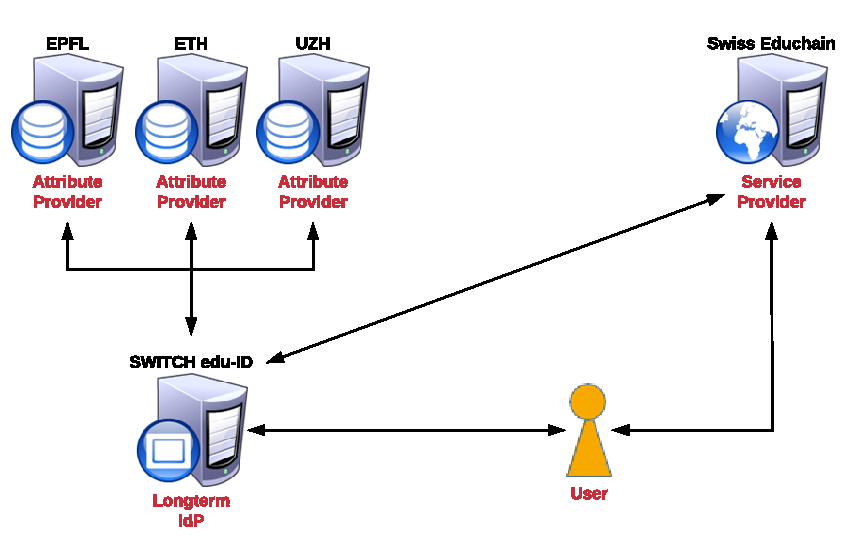
\includegraphics[width=0.6\textwidth]{figs/ch4/iam-diagram}
	\caption{SWITCH-Swiss Educhain architecture based on \cite{switch-eduid-architecture-presentation}.}
	\label{fig:iam-diagram}
\end{figure}

In Figure \ref{fig:iam-diagram} the high-level IAM architecture between Swiss Educhain, SWITCH edu-ID and the Attribute Providers is shown. The user only has a single unique long term identity, hosted and operated by SWITCH edu-ID, which can be used to create affiliation(s) with one or more Organizations. The Organizations act as attribute providers and attest that a certain individual has a specific role. Service Providers become members of the federation and register as Resources in the SWITCH AAI Resource Registry. Based on the approved Resource description and after the user's disclosure consent, only the required attributes are sent to the Service Provider by the edu-ID IdP. Attribute values are always fetched in real-time from all Attribute Providers and updated if needed before sent to the Service Provider. Figure \ref{fig:switch-resource-registry} depicts an overview of the Resource Registry tool. 

\begin{figure}[ht!]
	\centering
	\captionsetup{width=.75\linewidth}
	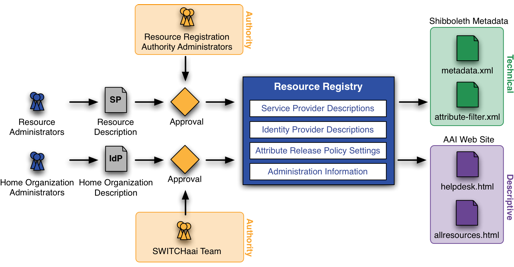
\includegraphics[width=0.75\textwidth]{figs/ch4/resource-registry}
	\caption{Resource Registry overview \cite{switch-resource-registry-info}.}
	\label{fig:switch-resource-registry}
\end{figure}

Swiss Educhain has registered as a Resource in the AAI Test federation with Home Organization the University of Zurich test IdP. For the architecture shown in Figure \ref{fig:iam-diagram} to be operational a certain level of trust needs to exist between the federation participants \cite{aai-federation}. Trust in this context refers to information or data  released from one federation participant to another, and that an entity trusts another means that the data (attributes) received are accepted as correct, complete and previously verified either directly from the data source or through a chain of trust. 



Figure \ref{fig:iam-trust-diagram} shows the trust relationships relative to the Swiss Educhain service. SWITCH edu-ID is the trusted root in the federation, thus trusted by everyone. There exists a two-way trust relationship between Attribute Providers and SWITCH edu-ID, a result of the gradually built trust during the onboarding of Organizations to the federation, a process that entails multiple steps and has a duration of several months \cite{eduid-adoption}. The identity data transferred are logically structured in the form of attributes. 

\begin{figure}[ht!]
	\centering
	\captionsetup{width=.75\linewidth}
	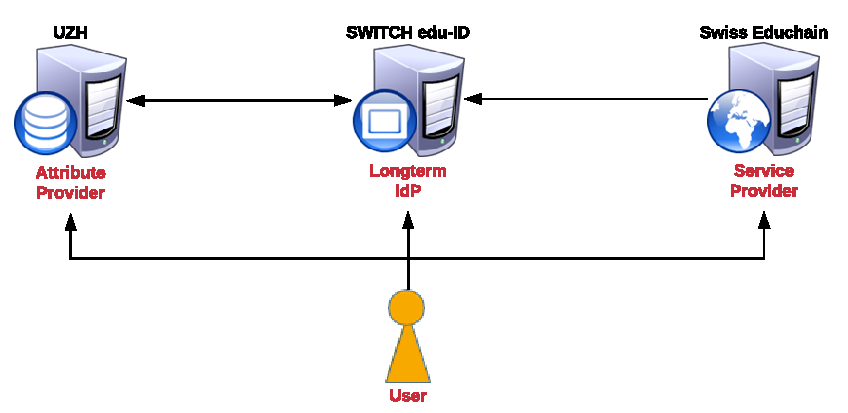
\includegraphics[width=0.6\textwidth]{figs/ch4/iam-trust-diagram}
	\caption{Swiss Educhain trust relationships.}
	\label{fig:iam-trust-diagram}
\end{figure}

Attributes are the main building block of SWITCH edu-ID and SWITCHaai identities. They offer a comprehensive and standardized way to structure user information and assist in simple attribute-based access control (ABAC) policy implementation, a concept previously introduced in Section \ref{ssec:access-control-models}. A SWITCH edu-ID identity consists of the following parts \cite{attribute-model}:

\begin{description}
	\itemsep0em
	\item\textbf{Personal part} - mandatory for all accounts, it must contain at least first name, last name and an email address.
	\item\textbf{Current affiliation} - added to an account when the user becomes a member of an organization (e.g. student or staff). May contain none, one or more current affiliations, and all current affiliations are created and managed by the respective organizations.
	\item\textbf{Former affiliation} - a current affiliation is transformed into a former affiliation when an individual leaves an organization. The set of former affiliations acts as the affiliation history of an individual.
	\item\textbf{Group memberships} - an identity's group memberships are represented in the \texttt{entitlement} attribute.
\end{description}

\begin{figure}[H]
	\begin{minipage}{0.49\linewidth}
		%\centering  % redundant
		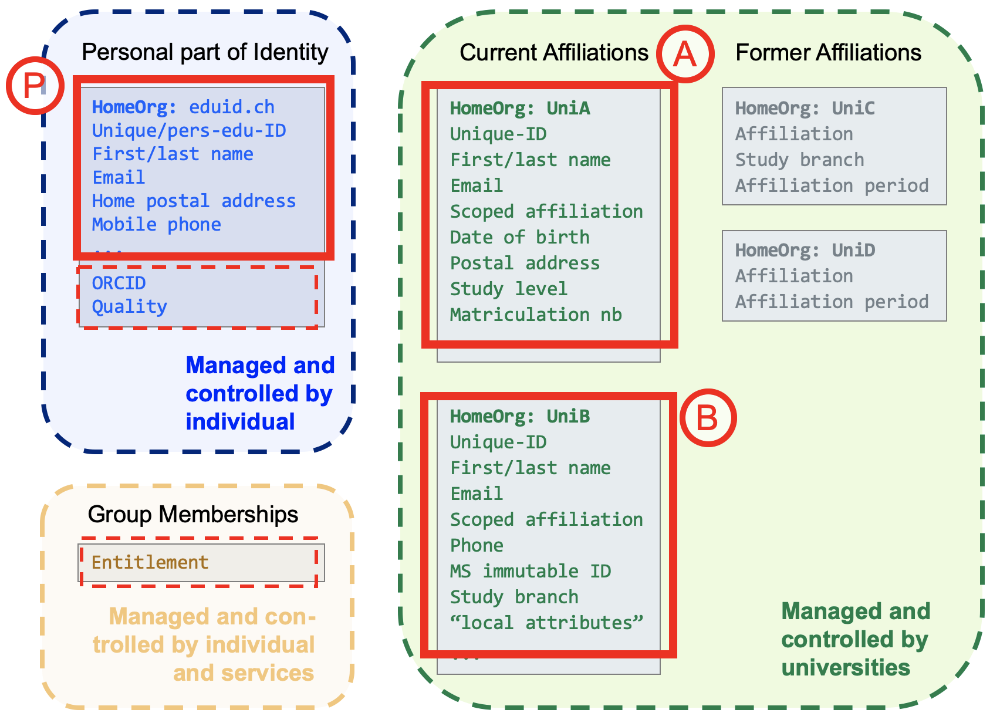
\includegraphics[width=\textwidth]{figs/ch4/classic-attribute-model}
	\end{minipage}%
	\hfill% not: "\hspace{0.5cm}"
	\begin{minipage}{0.49\linewidth}
		%\centering  % redundant
		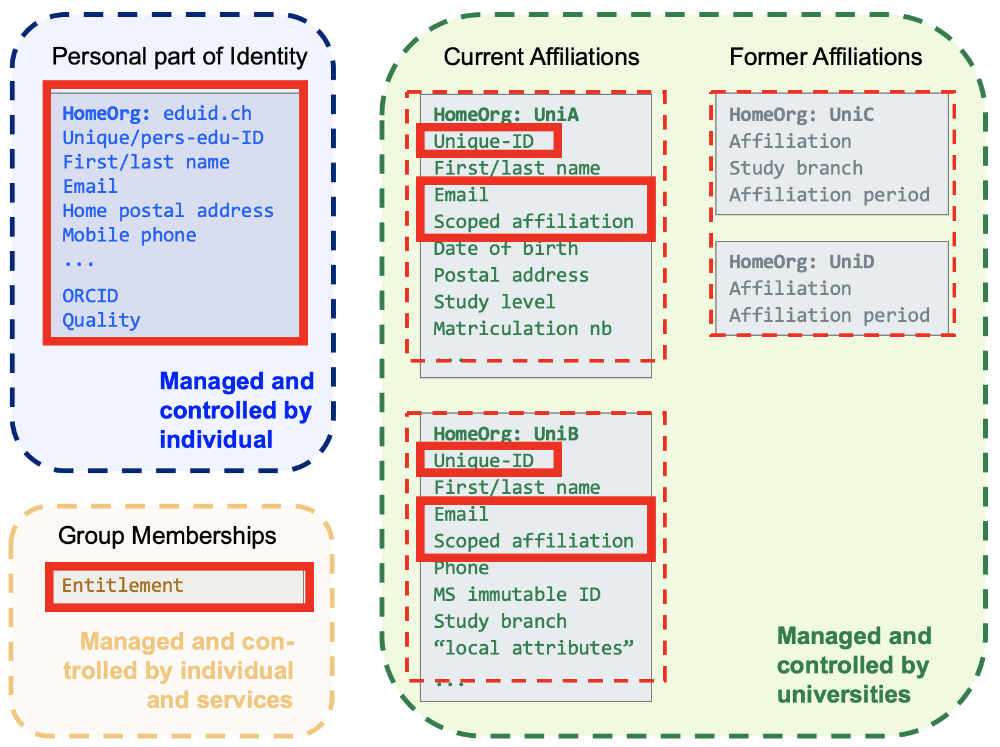
\includegraphics[width=\textwidth]{figs/ch4/extended-attribute-model}
	\end{minipage}
	\caption{Classic and Extended Attribute models for Service Providers \cite{classic-attribute-model}, \cite{eduid-extended-attribute-model}.}
	\label{fig:attribute-models}
\end{figure}

The differences in the way a Service Provider can request, and access user attributes is shown in Figure \ref{fig:attribute-models}. In the classic model, the service would either get the attribute assertion A or B, depending on the user's choice in the discovery service or the affiliation selection, a service can get only one part at a time. There may be cases where a service requires attributes from multiple home organizations simultaneously. This is possible in the extended model, where a service can potentially get a SAML assertion for attributes in the small bold red boxes in different parts of the identity. Swiss Educhain is using the extended model because it needs to fetch all current scoped affiliations (\texttt{swissEduIDLinkedAffiliation} attribute) of the users. Users login with their edu-ID account and all the attributes that are requested by Swiss Educhain are updated with the current values and then disclosed. The extended model login flow is shown in Figure \ref{fig:eduid-login-flows} and contrasted side by side with the classic model, where an affiliation is chosen before logging into a service.

\begin{figure}[ht!]
	\centering
	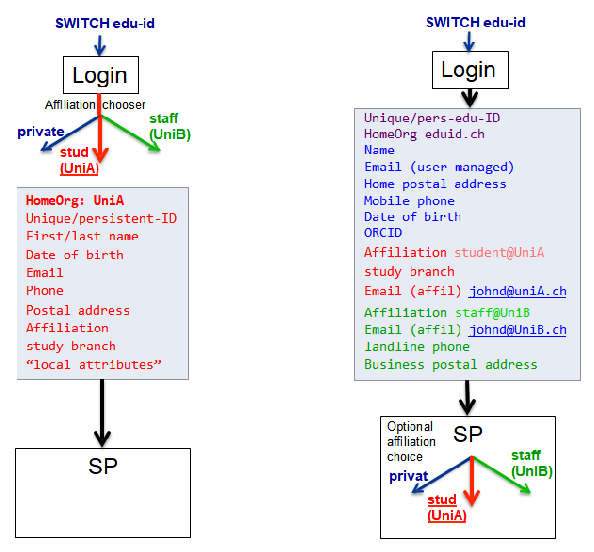
\includegraphics[width=0.75\textwidth]{figs/ch4/login-flows}
	\caption{Classic and Extended models login flows \cite{switch-eduid-services-presentation}.}
	\label{fig:eduid-login-flows}
\end{figure}

The two distinct roles that can be assumed by the Swiss Educhain service users are \textbf{Issuer} and \textbf{Recipient}. In order to be able to distinguish amongst two kinds of users and issue a diploma the following attributes must be disclosed:

\begin{description}
	\itemsep0em
	\item\textbf{commonName (cn)} - user's common name (first name, last name).
	\item\textbf{mail} - preferred email address to be used to send messages to this person.
	\item\textbf{matriculationNumber} - the unique long-lived matriculation number of a student.
	\item\textbf{swissEduIDLinkedAffiliation} - a list of organizational scoped-affiliations (e.g. student@uzh.ch, staff@ethz.ch).
	\item\textbf{persistentID} - a privacy-preserving user identifier shared between the Identity Provider (IdP) and the Service Provider (SP).
\end{description}

\subsection{Persistent ID} \label{persistent-id}

The persistentID attribute is generated by the IdP when the user accesses a specific SP for the first time. It is stored in a relational database when the IdP is configured as the SWITCHaai deployment guides instruct. If no database is configured, a new value will be computed every time using the predefined salt. As it is persistent, the value remains the same for all further sessions between the same user and the same Service Provider. For different Service Providers, different Persistent IDs are generated for a given user. Therefore, the Persistent IDs cannot be used to correlate user data, even if several Service Providers tried to aggregate data. This results in better user privacy \cite{persistent-id}.

%Add the expert demo diagram and just explain this shows the aai flow, but the edu-id flow is the same without the discovery service. The discovery service was used in aai to discover the home organisation and perform the authorization and attribute retrieval from the Organization IdP. In Edu-Id it is simpler as the IdP is defined during the integration with Shibboleth and is the unique Switch edu-ID IdP, which then updates all attributes by requesting the from the Attribute Authorities (previous IdPs in aai)
%https://www.switch.ch/aai/demo/expert/



\subsection{Target Audience} \label{ssec:iam-target-audience}

The target audience of the Swiss Educhain service is considered to be any edu-ID user which has at least one linked affiliation and a matriculation number. Linked affiliations are affilitations between edu-ID users and Organizations (acting as Attribute Providers), and should not be confused with the plain \texttt{affiliation} attribute which is the affiliation between a user and SWITCH edu-ID directly. 

\subsection{Role Assignment} \label{ssec:iam-role-assignment}

The activities of role assignment, management and revocation are outside of the Swiss Educhain system boundary. Roles should be strictly assigned and managed by the organizations, it is their sole responsibility to ensure that only the correct users are assigned the corresponding affiliation(s) which are interpreted by Swiss Educhain into the two distinct roles of \texttt{Issuer} and \texttt{Recipient}. Through the edu-ID IdP, Swiss Educhain is always provided with the latest up to date values of all the user account attributes. The most important attribute is \texttt{swissEduIDLinkedAffiliation} which holds all the current active user affiliations with one or more organizations, the values should only be present while the affiliation lasts, as soon as a user leaves an organization the affiliation should be marked as a former affiliation by edu-ID and the value removed from the attribute.

\subsection{User Access Control} \label{ssec:iam-access-control}

A user has different interactions and relationships with the \textbf{Service Provider} (Swiss Educhain), the \textbf{Identity Provider} (SWITCH edu-ID) and the \textbf{Attribute Provider(s)} (Organization(s)). In Figure \ref{fig:login-sequence} the login sequence steps are shown for a new session, this includes the different levels of access controls with the SP and the IdP. Even though the User Experience is excellent and the Web SSO works seamlessly, there are a lot of prerequisites, established processes and well-defined steps happening in the background to ensure privacy, security and verifiability.

\begin{figure}[h]
	\centering
	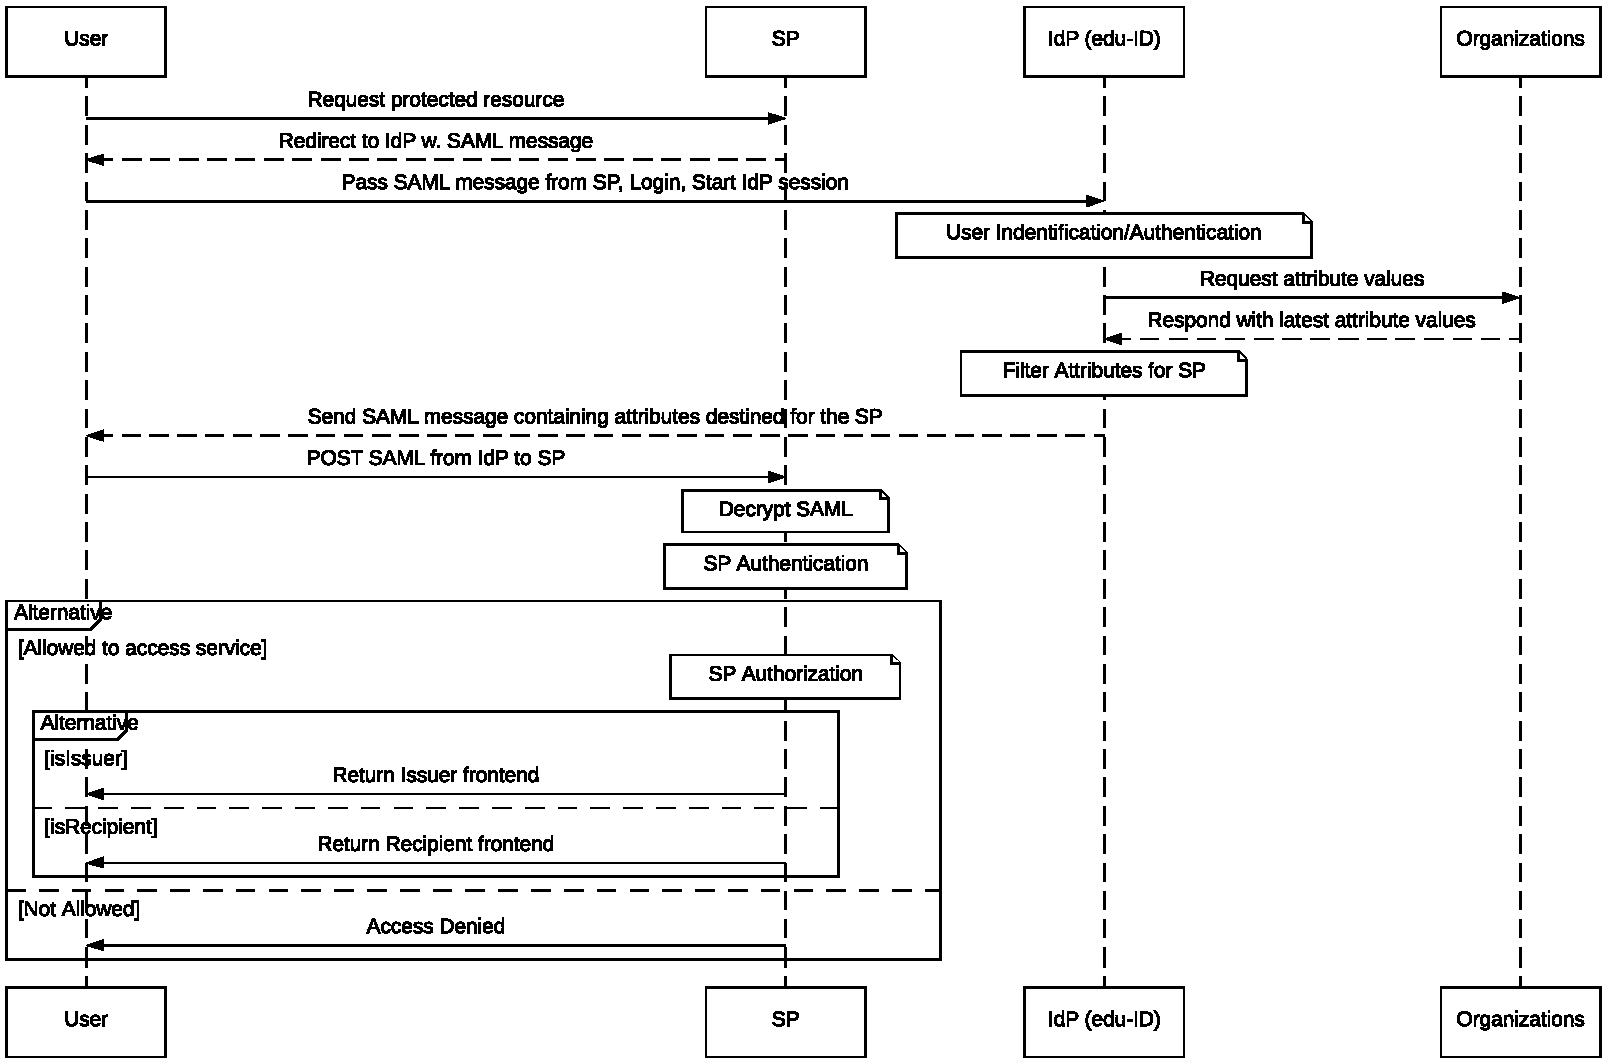
\includegraphics[width=\textwidth]{figs/ch4/login-sequence}
	\caption{Swiss Educhain login sequence diagram based on \cite{shib-logins}.}
	\label{fig:login-sequence}
\end{figure}

Initially, the user tries to visit the Swiss Educhain service (\url{https://educhain.csg.uzh.ch/app/}), the \texttt{mod\_shib} Apache module in the SP checks if a valid session exists to access the protected location relative to the base url (e.g. \textbf{/app/}), details on the implementation are provided at Chapter \ref{ch:implementation}. Since there is no active session the user is redirected to the IdP to login and authenticate, carrying also a SAML message from the SP which requests certain attributes. In other federated Web SSO scenarios the SP conducts a WAYF (Where Are You From) step to discover the IdP which holds the user's identity, while in the SWITCH edu-ID scenario the IdP is unique and already known to the SP (\url{https://login.test.eduid.ch/}). \\
The user reaches the IdP and needs to perform the identification and authentication steps (usually using a username and password). After the user successfully authenticates, the IdP updates all the attributes and linked affiliations of the user by sending requests to the Organizations that act as Attribute Providers. Once all the attributes have been received, the IdP performs any necessary updates internally and then consults the Resource Registry, to filter the attributes based on the SP Resource Description and the active Attribute Release Policy Settings. Then, the SAML response is encoded and sent back to the user to be forwarded to the SP, this response only contains the attributes that the SP is allowed to request and that are available. The user is shown a comprehensive message of which attributes will be disclosed to the SP. After providing consent, the SAML response is forwarded to the SP together with a new request to access the protected resource. \\
The SP decrypts the message, verifies the IdP signature and depending on the ABAC policy in effect, allows or denies access to the resource. User identification is done with the \texttt{persistentID} to preserve privacy, and authentication is inherited from the authentication statement produced by the IdP (possibly also stating if it was 1FA, 2FA or MFA). \\
Swiss Educhain has two levels of authorization, the service-level authorization which determines if a user should be granted access to the service in general and the application-level authorization which determines what actions the user will be allowed to perform. A detailed description is provided below.


\subsection{Authorization Policy} \label{ssec:educhain-authorization-policy}

\begin{description}
	\item\textbf{Service-Level Authorization} \hfill \\
	The service level policy is stored in the Apache Webserver configuration and uses the \texttt{mod\_shib} module (which integrates the local Shibboleth daemon with Apache) to check the received values and enforce the policy. 
	
	\textbf{Rules:} (Require All)
	\begin{description}
		\item\textbf{Valid Session} \hfill \\
		A valid shibboleth session needs to be active between the SP and the user, this means the user has authenticated with the IdP, the SP has validated the received authentication statement and a new session was created. 
		\item\textbf{Linked Affiliation exists} \hfill \\
		At least one linked affiliation exists, checked through the \texttt{swissEduIDLinkedAffiliation} attribute which needs to have at least one value.
		\item\textbf{Matriculation number exists} \hfill \\ 
		The user's matriculation number needs to be present and valid; the validity and non-duplication is ensured by SWITCH edu-ID. Attribute \texttt{matriculationNr} holds the value. In Swiss academia the matriculation number is only generated once and is used across organizations when needed.
	\end{description}

	If all the above conditions are true, Apache creates a session and sends a request to the Spring Boot embedded Tomcat server through the AJP protocol as shown in Figure \ref{fig:arch-educhain}. If any of the conditions is not satisfied access is denied and the user is redirected to an error page by the Shibboleth handler.
	
	\item\textbf{Application-Level Authorization} \hfill \\
	The application level policy only determines the role the user will assume. The two distinct application roles are \textbf{Issuer} and \textbf{Recipient} as defined in Section \ref{sec:stakeholders}.
	It must be clarified, as mentioned in detail in Section \ref{ssec:iam-role-assignment}, that Swiss Educhain does not manage any user accounts nor is able to assign access rights or affiliations on behalf of any Organization.

	\textbf{Rules:}
	\begin{description}
		\item\textbf{Recipient} \hfill \\
		\texttt{Recipient} is the role that is assigned by default to all the users that have access to the service. There is no additional check to verify that a user should assume the role of a \texttt{Recipient}, this is ensured from the check performed by Shibboleth and Apache.
		\item\textbf{Issuer} \hfill \\
		An \texttt{Issuer} has elevated access rights and is able to issue diplomas to one or more \texttt{Recipients} individually or in batch. To identify someone as an \texttt{Issuer} the CorDapp checks the \texttt{swissEduIDLinkedAffiliation} attribute for the values \texttt{staff@uzh.ch} or \texttt{faculty@uzh.ch}. For the Swiss Educhain to be released to production and Organizations to be able to assign the role of \texttt{Issuer} a new value should be available in the \texttt{swissEduIDLinkedAffiliation} attribute, \texttt{issuer} (e.g. \texttt{issuer@uzh.ch, issuer@epfl.ch}). The values of \texttt{staff} and \texttt{faculty} are used for the purpose of the MVP implementation.
	\end{description}

	A view of the frontend interface is shown in Figure \ref{fig:educhain-frontend} in Chapter \ref{ch:implementation}.
\end{description}


\subsection{Application Accounts} \label{ssec:iam-application-accounts}

The extensive integration with SWITCH edu-ID has been described and the solution design has been presented. It is essential to define the mapping amongst edu-ID identities with Swiss Educhain application accounts. Figure \ref{fig:identity-mapping} shows the information flow and granular identity mapping of parts for the various entities.

\begin{figure}[H]
	\centering
	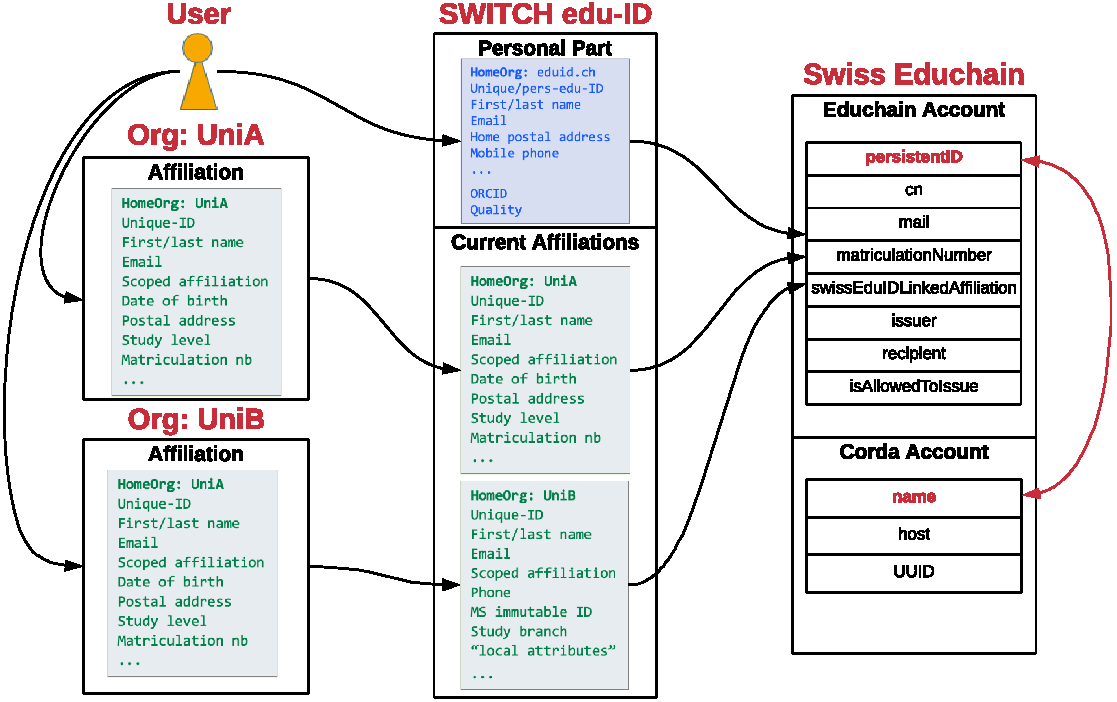
\includegraphics[width=\textwidth]{figs/ch4/identity-mapping}
	\caption{Information flow and identity mapping.}
	\label{fig:identity-mapping}
\end{figure}

\begin{description}
	\item\textbf{User} \hfill \\
	The user provides personal and contact information to the affiliated Organizations and the edu-ID IdP. Information provided by the user is not trusted by default and must be always verified, either digitally or via in-person verification. The user owns and manages the personal part of the edu-ID account, following a user-centric approach.
	\item\textbf{Organizations} \hfill \\
	Organizations no longer act as a complete identity provider which hosts and manages the users' accounts. In the edu-ID architecture, they host only the affiliations that exist with users, entrusting the user identity management responsibility to edu-ID. Thus, they act as Attribute Providers to edu-ID, by assigning individual roles and access rights using the attribute values. In other use cases, the relationship with edu-ID can be two way, but from Swiss Educhain's perspective the flow of information is only unidirectional. 
	\item\textbf{edu-ID IdP} \hfill \\
	Edu-ID is the central root of trust of the SWITCH federation and is the sole IdP, serving all the other entities. Edu-ID acts as a data provider and a source of trust for Swiss Educhain. It provides only the relevant (and approved for release) parts or attributes of a user's identity to the service. Apart from the information depicted, edu-ID holds a wide variety of metadata and a history of all the former affiliations of a user.
	\item\textbf{Swiss Educhain} \hfill \\
	Swiss Educhain acts solely as a consumer of information from a single data source, the edu-ID IdP. A strong trust relationship is assumed, to treat all user data disclosed as authentic, complete and valid. Internally, specific attributes are used to provide two levels of authorization and identify a user (persistentID). A Corda account is created to be used in transactions and is logically mapped one-to-one with the EduchainAccount. The Educhain account is stored as a Corda state with specific attributes and is updated if needed after every login. The \texttt{persistentID} attribute acts as the primary key and is used to perform all account related activities. More information on the implementation of accounts is provided at Chapter \ref{ch:implementation}.
\end{description}